\documentclass{bioinfo}
\copyrightyear{2013}
\pubyear{2013}

\usepackage{fixltx2e}
\usepackage{natbib}
\bibliographystyle{apalike}

\newcommand{\textssf}[1]{\textsf{\footnotesize #1}}

\begin{document}
\firstpage{1}

\title{}

\author[Li]{Heng Li}

\address{Broad Institute of Harvard and MIT, 7 Cambridge Center, Cambridge, MA 02142, USA}

\history{Received on XXXXX; revised on XXXXX; accepted on XXXXX}
\editor{Associate Editor: XXXXXXX}
\maketitle

\begin{abstract}

Indel realignment and BQSR are not critical for deep resequencing with 100bp
HiSeq data. The accuracy of SNP callers vary with mappers. Most SNP callers
work better with bwa-mem. No single pipeline clearly outperforms all the
others.

\end{abstract}

\section{Results}

\begin{table*}
\footnotesize
\processtable{Evaluated mappers and variant callers}
{\begin{tabular*}{\textwidth}{@{\extracolsep{\fill}}lllp{12cm}}
\toprule
Symbol & Algorithm & Version & Command line \\
\midrule
bt2 & bowtie2 & 2.1.0 & bowtie2 -x \emph{ref.fa} -1 \emph{read1.fq} -2 \emph{read2.fq} -X 500 \\
bwa & bwa-backtrack & 0.7.6 & bwa aln -f \emph{read1.sai} \emph{ref.fa} \emph{read1.fq}; bwa sampe \emph{ref.fa} \emph{read1.sai} \emph{read2.sai} \emph{read1.fq} \emph{read2.fq} \\
mem & bwa-mem & 0.7.6 & bwa mem \emph{ref.fa} \emph{read1.fq} \emph{read2.fq} \\
fb & freebayes & 0.9.9 & freebayes -f \emph{ref.fa} \emph{aln.bam} \\
st & samtools & 0.1.19+ & samtools mpileup -Euf \emph{ref.fa} \emph{aln.bam} {\tt \char124} bcftools view -v - \\
st-noBAQ & samtools & 0.1.19+ & samtools mpileup -Buf \emph{ref.fa} \emph{aln.bam} {\tt \char124} bcftools view -v - \\
sta & samtools & 0.1.19+ & samtools mpileup -ZBuf \emph{ref.fa} \emph{aln.bam} {\tt \char124} bcftools view -v - \\
ug & UnifiedGenotyper & 2.7-4 & java -jar GenomeAnalysisTK.jar -T UnifiedGenotyper -R \emph{ref.fa} -I \emph{aln.bam} \mbox{-stand\_call\_conf 30} \mbox{-stand\_emit\_conf 10} \\
hc & HaplotypeCaller & 2.7-4 & java -jar GenomeAnalysisTK.jar -T HaplotypeCaller --genotyping\_mode DISCOVERY -R \emph{ref.fa} -I \emph{aln.bam} \mbox{-stand\_call\_conf 30} \mbox{-stand\_emit\_conf 10} \\
pt & Platypus & 0.5.2 & Platypus.py callVariants --bamFiles=\emph{aln.bam} --refFile=\emph{ref.fa} \\
\botrule
\end{tabular*}}{}
\end{table*}

\subsection{The transition-to-transversion ratio of SNPs}
Transitions refer to {\tt A}$\Leftrightarrow${\tt G} or {\tt
C}$\Leftrightarrow${\tt T} substitutions, while transversions refer to other
types of substitutions. Because there are 8 types of transversions but only 4
types of transitions, we would expect to see the ratio of transitions to
transverions (ts/tv) is 0.5 if substitutions are independent of compositions.
However, biologically, transitions occur more easily. Ts/tv is frequently much
larger. For example, ts/tv of human-chimpanzee substitutions is 2.08 on
autosomes based on Ensembl's EPO alignment v50, or 1.97 based v62. If we assume
human SNPs arose in a similar biological process, ts/tv of SNPs should be
around 2 as well.

\subsection{Effect of mapper-caller combinations}

Fig~\ref{fig:qroc1} shows ts/tv as a function of the accumulative number of
SNPs, stratified by the SNP quality. If we assume ts/tv to be an indicator of
FPR, we have the following observations.

\begin{figure}[!hp]
\centering\includegraphics[width=.4\textwidth]{qst2/qroc-CHM1-bt2}\\
\centering\includegraphics[width=.4\textwidth]{qst2/qroc-CHM1-mem}
\caption{Effect of the combination of mappers and SNP callers. SNPs are sorted
by their reported qualities in the descending order and evenly divided into 20
bins. Each dot gives the transition-to-transversion ratio (ts/tv) of SNPs in a
bin and the accumulative number of SNPs up to the bin.}\label{fig:qroc1} \end{figure}

Firstly, \textssf{ug}, \textssf{hc} and \textssf{st} callers have similar
accuracy given the same alignment and they tend to call more SNPs from the
\textssf{mem} and \textssf{bwa} alignments than from \textssf{bt2} at similar
ts/tv. To understand this, we extracted 155k Q100 SNPs from \textssf{mem:hc}
that are absent from unfiltered \textssf{bt2:hc}. Interestingly, the vast
majority of these SNPs are visiable in the \textssf{bt2} alignment, but the
mapping quality (mapQ) of non-reference reads is consistently lower -- the
median of the per-site mapQ average is 8 in \textssf{bt2} vs. 30 in \textssf{mem}.
For \textssf{st}, \textssf{ug} and \textssf{hc}, the actual quality used in
variant calling is the smaller between base quality and mapQ. The low mapQ
prevents them from calling these SNPs from the \textssf{bowtie2} alignment.
Looking at the alignment in an alignment viewer, we think \textssf{bowtie2} is
usually conservative on mapQ, but we also spot cases where bwa-mem is
overconfident in mappings with excessive substitutions. Neither mapper gives
ideal results.

A second observation is that \textssf{freebayes} is less sensitive to mappers and it
consistently calls more SNPs than other callers. This is also caused by the way
mapQ is used by the callers. We extracted 162k Q100 SNPs from \textssf{mem:fb}
that are absent from unfiltered \textssf{mem:hc}. 28\% of them are only
supported by reads with repetitive mappings, which strongly suggests that
\textssf{freebayes} ignores mapQ during variant calling and is thus more likely
to take differences between copies of segmental duplications as variants. As
substitutions between copies of duplications also follow the same mutation
process, their ts/tv should not be much different from the ts/tv of SNPs. This
could explain why \textssf{freebayes} calls more SNPs than others at similar
ts/tv. As the major difference between \textssf{bowtie2} and \textssf{bwa-mem}
is the estimate of mapQ, ignoring mapQ also makes them more comparable.

It is worrying that mapQ has a big impact on the results.

\subsection{Effect of indel realignment and base recalibration}

\begin{figure*}[!hp]
\centering\includegraphics[width=.4\textwidth]{qst2/qroc-NA12878-bt2}
\centering\includegraphics[width=.4\textwidth]{qst2/qroc-NA12878-bwa}\\
\centering\includegraphics[width=.4\textwidth]{qst2/qroc-NA12878-mem}
\centering\includegraphics[width=.4\textwidth]{qst2/qroc-realn-bqsr}
\caption{Effect of indel realignment and base recalibration.}\label{fig:qroc2} \end{figure*}

%\begin{figure}[!hp]
%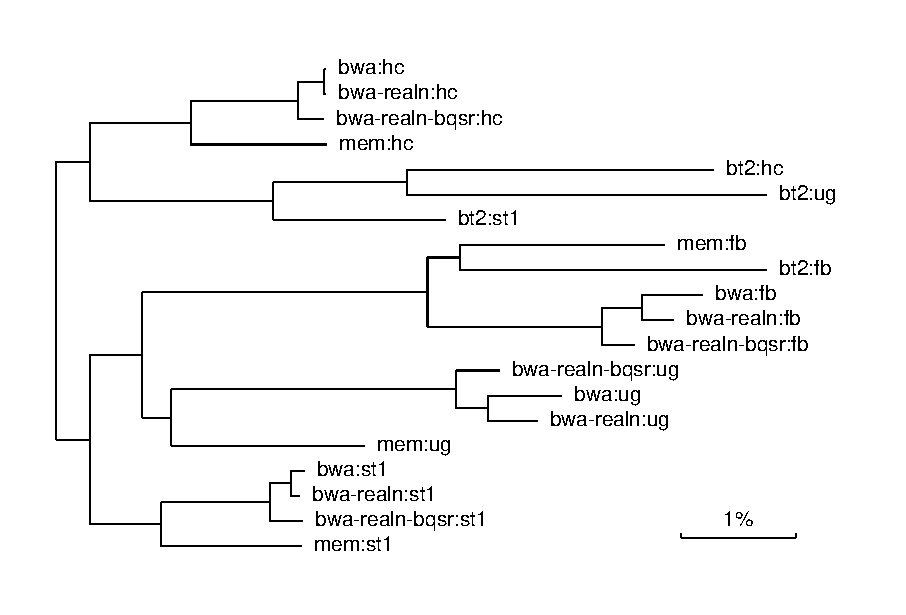
\includegraphics[width=.49\textwidth]{tree}
%\label{fig:tree} \end{figure}

\begin{table*}
\processtable{Relation between call sets}
{\begin{tabular*}{\textwidth}{@{\extracolsep{\fill}}lcccccccccccc}
\toprule
 & bt2:fb & bwa:fb & bwa:hc & bwa:pt & bwa:st1 & bwa:ug & mem:fb & mem:hc & mem:pt & mem:st & mem:sta & mem:ug \\
\midrule
bt2:fb & {\bf 3831839} & {\bf 0.975}/1.5 & 0.920/1.6 & 0.928/1.6 & 0.933/1.5 & 0.925/1.6 & {\bf 0.970}/1.5 & 0.928/1.6 & 0.931/1.6 & 0.938/1.5 & 0.966/1.5 & 0.930/1.6 \\
bwa:fb & {\bf 0.977}/1.3 & {\bf 3826595} & 0.923/1.6 & 0.934/1.6 & 0.938/1.4 & 0.932/1.6 & {\bf 0.972}/1.4 & 0.929/1.6 & 0.933/1.6 & 0.938/1.5 & 0.967/1.5 & 0.932/1.6 \\
bwa:hc & 0.984/0.9 & 0.985/0.9 & {\bf 3583492} & 0.984/1.5 & 0.980/0.9 & 0.980/1.5 & 0.982/1.0 & {\bf 0.993}/1.6 & 0.982/1.4 & 0.979/1.0 & {\bf 0.990}/1.3 & 0.981/1.3 \\
bwa:pt & 0.973/1.0 & {\bf 0.978}/0.9 & 0.966/1.3 & {\bf 3652743} & 0.966/1.0 & {\bf 0.975}/1.4 & 0.970/1.0 & 0.963/1.3 & {\bf 0.977}/1.4 & 0.962/1.1 & {\bf 0.979}/1.3 & 0.969/1.3 \\
bwa:st1 & {\bf 0.990}/1.2 & {\bf 0.993}/1.1 & 0.972/1.6 & 0.977/1.7 & {\bf 3612146} & 0.974/1.7 & 0.987/1.3 & 0.974/1.6 & 0.976/1.6 & {\bf 0.990}/1.6 & {\bf 0.989}/1.4 & 0.976/1.5 \\
bwa:ug & 0.977/0.7 & {\bf 0.983}/0.6 & 0.968/1.1 & {\bf 0.981}/1.0 & 0.970/0.8 & {\bf 3628793} & 0.975/0.8 & 0.966/1.1 & 0.974/1.1 & 0.966/0.9 & {\bf 0.986}/0.9 & 0.980/1.0 \\
mem:fb & {\bf 0.984}/1.5 & {\bf 0.985}/1.6 & 0.932/1.6 & 0.938/1.7 & 0.944/1.5 & 0.937/1.7 & {\bf 3775292} & 0.942/1.6 & 0.946/1.7 & 0.953/1.5 & {\bf 0.985}/1.5 & 0.946/1.6 \\
mem:hc & 0.985/0.9 & 0.984/0.9 & 0.985/1.7 & 0.974/1.5 & 0.974/1.1 & 0.971/1.6 & 0.984/0.9 & {\bf 3612515} & 0.984/1.4 & 0.980/0.9 & {\bf 0.992}/1.2 & 0.981/1.4 \\
mem:pt & 0.983/0.9 & 0.983/0.9 & 0.969/1.4 & 0.983/1.6 & 0.971/1.0 & 0.973/1.5 & 0.984/0.8 & 0.978/1.3 & {\bf 3631994} & 0.976/0.9 & {\bf 0.994}/1.2 & 0.984/1.2 \\
mem:st & {\bf 0.992}/1.2 & {\bf 0.991}/1.4 & 0.968/1.7 & 0.970/1.7 & 0.987/1.7 & 0.968/1.7 & {\bf 0.994}/1.2 & 0.978/1.7 & 0.979/1.7 & {\bf 3621684} & {\bf 0.996}/1.2 & 0.979/1.6 \\
mem:sta & {\bf 0.975}/1.0 & 0.974/1.1 & 0.934/1.5 & 0.942/1.6 & 0.941/1.3 & 0.942/1.6 & {\bf 0.980}/0.9 & 0.944/1.5 & 0.951/1.6 & 0.950/1.2 & {\bf 3797069} & 0.952/1.6 \\
mem:ug & 0.985/0.9 & 0.986/0.9 & 0.971/1.4 & 0.978/1.6 & 0.974/1.0 & 0.983/1.7 & 0.987/0.8 & 0.979/1.3 & 0.987/1.5 & 0.979/0.9 & {\bf 0.998}/1.4 & {\bf 3619760} \\
\botrule
\end{tabular*}}{}
\end{table*}

\end{document}
